
\chapter{Introduction}
\label{ch:introduction}

Physical AI controllers---battery dispatch optimisers, autonomous-vehicle
planners, robotic manipulators---share a structural assumption so pervasive
that it is rarely stated explicitly: \emph{the observation available to the
controller faithfully represents the physical state of the plant.}  This
dissertation investigates what happens when that assumption fails, using
grid-scale battery energy storage systems (BESS) as the first rigorous
validation surface.

\section{The Hidden Assumption in Physical AI}

Every feedback controller closes a loop: sense the plant state, compute an
action, actuate, repeat.  Classical control theory formalises this loop with
a state vector~$x_t \in \mathcal{X}$, a measurement function~$h$, and an
observation~$y_t = h(x_t) + v_t$, where $v_t$ is zero-mean sensor noise.
When the noise is well-characterised---Gaussian, bounded, independent---the
Kalman filter or its nonlinear descendants recover the true state with known
error bounds, and the controller can act as if it sees the truth.

Modern cyber-physical systems (CPS) break this contract in ways that are
neither Gaussian nor bounded.  Telemetry arrives over packet-switched
networks subject to dropout, delay, replay, and stale-sensor failure.
The resulting observation~$\hat{x}_t$ is not simply $x_t$ plus noise;
it may be \emph{structurally incorrect}: the controller sees a state that
the plant never occupied.  No amount of Kalman filtering can correct for a
reading that was dropped entirely and replaced by an interpolated hold.

The consequence is subtle but dangerous.  The controller evaluates its
safety constraints against $\hat{x}_t$, not $x_t$.  If $\hat{x}_t$
satisfies the constraints, the controller judges the situation safe.
Meanwhile, the true state~$x_t$ may already violate a physical limit.
The system is \emph{observationally safe} but \emph{physically unsafe}---a
condition we call the \emph{Observation-Action Safety Gap} (OASG).

\section{Why Observed Safety Can Differ from Physical Safety}

Consider a battery dispatched at 50\% SOC (state of charge).  A telemetry
packet carrying the latest voltage and current readings is delayed by two
intervals.  The controller still sees SOC~$= 50\%$ and issues a large
discharge.  In reality, a prior discharge already pushed SOC to 22\%.
The new action drives the physical SOC below the 20\% safety floor.
The observed trajectory shows no violation; the true trajectory shows a
hard constraint breach.  Figure~\ref{fig:oasg-hero} illustrates this
gap and the five-stage DC3S pipeline that closes it.

\begin{figure}[htbp]
\centering
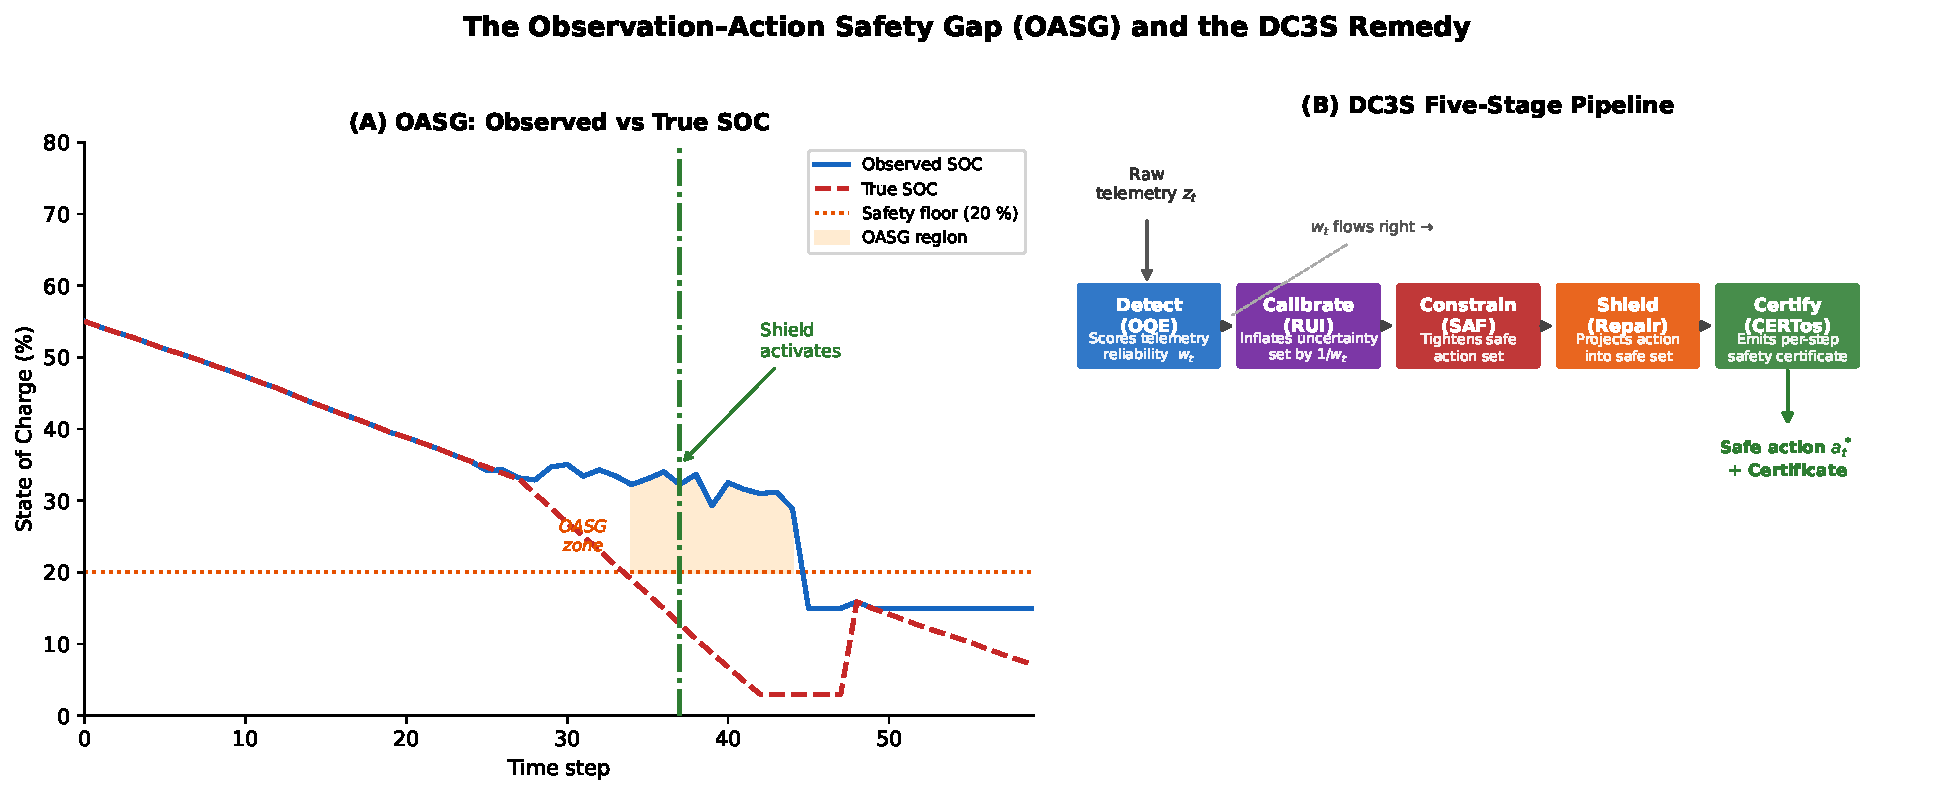
\includegraphics[width=0.95\linewidth]{paper/assets/figures/fig_oasg_hero}
\caption{The OASG in practice (left): observed SOC appears above the 20\%
safety floor while the true SOC has already breached it.  DC3S detects
reliability degradation, inflates the safety margin, and intercepts the
unsafe action before dispatch.  The DC3S five-stage pipeline (right)
maps the live OQE reliability score $w_t$ through calibrated uncertainty
inflation (RUI), tightened action constraints (SAF), safe-action repair,
and auditable runtime certificates (CERTos).}
\label{fig:oasg-hero}
\end{figure}

This is not a contrived edge case.  Field telemetry from US-grid EIA-930
data exhibits dropout rates of 5--15\% under normal operation and exceeding
30\% during storm events.  Germany's ENTSO-E feeds show comparable
patterns with additional regulatory delay.  Every dropped, delayed, or
stale reading widens the gap between observation and truth.

\section{The Observation-Action Safety Gap}
\label{sec:intro-oasg}

We define the OASG as the divergence between a controller's safety
assessment on its observed state and the actual safety status of the
physical plant:

\begin{definition}[Observation-Action Safety Gap (OASG)]
\label{def:oasg-informal}
Let $\hat{x}_t$ be the controller's observation and $x_t$ the true
state.  The \emph{OASG} at time~$t$ is the event
\[
  \mathcal{G}_t \;=\;
  \bigl\{\,a_t \in \mathcal{A}(\hat{x}_t)\;\bigr\}
  \;\cap\;
  \bigl\{\,a_t \notin \mathcal{A}(x_t)\;\bigr\},
\]
where $\mathcal{A}(x)$ denotes the set of actions satisfying all safety
constraints at state~$x$.  When $\mathcal{G}_t$ is non-empty, the
controller has chosen an action that appears safe on the observation
but violates constraints on the truth.
\end{definition}

The OASG is \emph{invisible} to any evaluation protocol that checks
constraints only on the observed trajectory.  Revealing it requires
maintaining a parallel \emph{true-state trajectory}---a dual-trajectory
architecture that is a cornerstone of the CPSBench harness developed in
this work (Chapter~\ref{ch:safety-illusion}).

\section{Why the Battery Domain Exposed the Problem First}

Batteries present three properties that make the OASG both acute and
measurable:

\begin{enumerate}
  \item \textbf{Hard state constraints.}  SOC must remain within
    $[\text{SOC}_{\min}, \text{SOC}_{\max}]$.  There is no elastic zone;
    violating the lower bound risks cell damage, and violating the upper
    bound risks thermal runaway.
  \item \textbf{High action-to-state sensitivity.}  A single dispatch
    decision at 50~MW for a 100~MWh battery moves SOC by 50\% in one hour.
    Even a brief observation error translates into a large true-state
    deviation.
  \item \textbf{Network-mediated telemetry.}  Grid-scale batteries are
    monitored via SCADA, cellular, or satellite links---all subject to the
    packet-level faults that create the OASG.
\end{enumerate}

Other CPS domains (autonomous vehicles, industrial robots) share
property~(3) but lack the clean measurability of~(1) and~(2).  The battery
domain is therefore the ideal \emph{first proving ground} for a general
theory of observation-aware safety.

\section{The ORIUS Principle}
\label{sec:orius-principle}

ORIUS---\textbf{O}bservation-\textbf{R}eliability--aware
\textbf{U}ncertainty-\textbf{I}nflated \textbf{S}afety---is the
organising principle of this dissertation.  It prescribes a four-stage
runtime pipeline:

\begin{enumerate}
  \item \textbf{Observation Quality Engine (OQE).}  Score the current
    telemetry reliability $w_t \in [w_{\min}, 1]$ using delay, freshness,
    spike, and stale-sensor features.
  \item \textbf{Reliability-aware Uncertainty Inflator (RUI).}  Inflate
    conformal prediction intervals by a factor proportional to $1/w_t$,
    widening the uncertainty set when observations are poor.
  \item \textbf{Safe-Action Filter (SAF).}  Tighten the feasible action
    set so that the dispatched action remains within SOC bounds even under
    worst-case realisations of the inflated uncertainty.
  \item \textbf{DC3S Shield.}  Issue a \emph{safety certificate} for
    every dispatched action, recording the observation quality, uncertainty
    bounds, and the margin to the nearest constraint.
\end{enumerate}

DC3S---the \textbf{D}ata-\textbf{C}entric \textbf{C}ertified
\textbf{C}onformal \textbf{S}hield---is the concrete realisation of the
ORIUS principle for the battery dispatch domain.

\section{Research Questions}

This dissertation addresses three central questions:

\begin{enumerate}
  \item[\textbf{RQ1.}] \emph{Does the Observation-Action Safety Gap exist
    in real-world battery dispatch?}  Specifically, do standard controllers
    (deterministic LP, robust MPC, stochastic risk-aware) produce actions
    that satisfy observed-state constraints while violating true-state
    constraints under realistic telemetry degradation?
  \item[\textbf{RQ2.}] \emph{Can a certificate-aware runtime safety layer
    close the gap?}  Can a lightweight online shield, informed by
    observation quality scores and conformal uncertainty, guarantee
    physical safety at the cost of bounded economic intervention?
  \item[\textbf{RQ3.}] \emph{What is the formal safety guarantee, and
    under what assumptions does it hold?}  Can we state a theorem of the
    form ``if telemetry faults satisfy bounds~$\mathcal{F}$ and the
    calibration set is exchangeable, then the true-state violation rate is
    at most~$\alpha$ with probability at least~$1 - \delta$''?
\end{enumerate}

\section{Contributions}

The principal contributions are:

\begin{enumerate}
  \item \textbf{Formalisation of the OASG.}  A rigorous definition of the
    gap between observed-state and true-state safety, together with a
    taxonomy of telemetry faults that create it
    (Chapter~\ref{ch:problem-formulation}).
  \item \textbf{The DC3S runtime shield.}  A four-stage pipeline (OQE,
    RUI, SAF, Shield) that closes the OASG with a provable coverage
    guarantee (Chapters~\ref{ch:safety-illusion}--\ref{ch:cert-half-life-blackout}).
  \item \textbf{CPSBench evaluation harness.}  A deterministic,
    dual-trajectory benchmark for battery dispatch under telemetry faults,
    enabling reproducible comparison of observation-aware controllers
    (Chapter~\ref{ch:orius-bench-battery}).
  \item \textbf{Empirical validation on US and DE grids.}  End-to-end
    experiments on EIA-930 (US) and ENTSO-E (Germany) data demonstrating
    zero true-state SOC violations across all tested dropout rates, with
    intervention rates below 20\%.
  \item \textbf{Extension results.}  Certificate half-life analysis
    (Chapter~\ref{ch:cert-half-life-blackout}), graceful degradation
    (Chapter~\ref{ch:graceful-degradation}), compositional fleet safety
    (Chapter~\ref{ch:compositional-safety-fleets}), and a CertOS runtime
    chapter that promotes the certificate lifecycle from roadmap language
    into bounded systems evidence (Chapter~\ref{ch:certos-runtime}).
\end{enumerate}

\section{Contribution Boundary}

This work does \emph{not} claim to solve the general partial-observability
problem for all CPS domains.  The safety guarantee is stated and validated
for the battery dispatch domain under the fault model of
Chapter~\ref{ch:problem-formulation}.  Extension to other domains
(e.g., autonomous driving, surgical robotics) requires domain-specific
instantiation of the OQE and SAF stages and is left to future work.

We also do not replace the upstream forecast or optimisation model.  DC3S
is a \emph{post-optimiser safety layer}: it takes the dispatch action
produced by any optimiser and certifies or corrects it before actuation.
The economic optimiser remains a black box to the shield.

\section{Organisation of the Manuscript}

The remainder of this dissertation is organised as follows:

\begin{description}
  \item[Chapter~\ref{ch:related-work}] surveys background and related work
    in battery dispatch, telemetry faults, conformal prediction, and
    runtime safety shields.
  \item[Chapter~\ref{ch:problem-formulation}] formalises the system model,
    fault model, SOC dynamics, the observation quality engine, and states
    the research questions mathematically.
  \item[Chapter~\ref{ch:safety-illusion}] defines the observed-state
    safety illusion and motivates the dual-trajectory evaluation paradigm.
  \item[Chapters~\ref{ch:assumptions}--\ref{ch:ablations}] develop the DC3S pipeline components, prove the
    coverage theorem, and present ablation studies.
  \item[Chapters~\ref{ch:cert-half-life-blackout}--\ref{ch:certos-runtime}]
    extend the framework to certificate temporal validity, graceful
    degradation, fleet composition, and certificate-aware runtime control.
  \item[Chapter~\ref{ch:orius-bench-battery}] describes the ORIUS-Bench
    battery track for reproducible benchmarking.
  \item[Chapter~\ref{ch:outside-current-evidence}] records bounded but
    intentionally non-promoted evidence surfaces, including the active
    probing audit and other claims that remain outside the defended core.
\end{description}
